\chapter{Einleitung}

Im Jahr 2022 veränderte OpenAI mit ihrem browserbasierten ChatGPT (Generative Pre-trained Transformer) \cite{openai_chatgpt_2022} die Welt komplett. In nur fünf Tagen erreichte ChatGPT eine Million Nutzer\*innen \cite{doit_software_chatgpt_2025} und ist aus dem Alltag vieler Menschen nicht mehr wegzudenken.
Die GPT-KI (Künstliche Intelligenz) von OpenAI gehört zur Familie der Large Language Models (LLMs) oder auch Multimodal Large Language Models (MLLMs). MLLMs können neben Text weitere Datenmodalitäten wie zum Beispiel Bilder, Audio und Video verarbeiten.
LLMs von anderen Anbietern wie Googles Gemini \cite{gemini_team_2023} und DeepSeek \cite{deepseek_team_2024} haben mit der Qualität und den Fähigkeiten von OpenAIs GPT gleichgezogen. Mittlerweile gibt es viele Arten, LLMs zu bewerten, und ein reger Wettbewerb ist um die vielen Bewertungen entstanden.

Die GPT-Modelle von OpenAI und anderen Anbietern wie Googles Gemini \cite{gemini_team_2024} sind meistens nur über eine API (Programmierschnittstelle) gegen Entgelt verfügbar.
Open-Source-Modelle wie DeepSeek \cite{deepseek_team_2024} oder Metas LLAMA \cite{touvron_2023} erfreuen sich immer größerer Beliebtheit, da sie gratis auf der eigenen Hardware ausgeführt werden können.

Im Oktober 2023 kam der Verfasser das erste Mal mit Retrieval-Augmented Generation (RAGs) in Kontakt; damals war die Idee, mit Hilfe eines LLMs Fragen über mehrere firmeninterne Informationsquellen zu beantworten.
Bei einem Hackathon gelang es dem Team des Verfassers, einen Prototypen (im folgenden System genannt) zu entwickeln, der mit einem gewissen Erfolg Fragen zu firmeninternen Themen beantworten konnte.

Einer der Schritte während der Entwicklung war das ständige Testen der neuesten Änderungen. Dadurch konnte die Funktionsfähigkeit überwacht und eventuelle schlechte Ergebnisse dokumentiert werden.
Diese zeitintensive Aufgabe kostete uns wertvolle Zeit, welche das Team lieber in die Entwicklung investiert hätte.
Gerne hätten wir unterschiedliche Prompts (Vorlagen von Fragen an ein LLM) innerhalb unseres Systems getestet oder eine automatische Überprüfung unserer neuesten Änderungen genutzt.

Ragas \cite{es_ragas_2024} wurde entwickelt, um diese Probleme zu lösen. Es hat zudem das Alleinstellungsmerkmal, dass man weder eigene Fragen noch die generierten Fragen selbst beantworten muss.
Sowohl die Generierung eines Fragenkatalogs (Testsets) als auch die Beantwortung der Fragen, um eine Musterlösung zu erstellen, nimmt RAGAS mithilfe von LLMs vor.
Mithilfe dieses Testsets und von RAGAS eigens entwickelter Metriken, welche die wichtigsten Funktionen eines RAGs abdecken, kann eine Bewertung des Systems vorgenommen werden.

Damit benutzt RAGAS die neue LLM-Technologie, um das durch LLMs entstandene System selbst zu testen. Dies spart menschliche Ressourcen, welche zeit- und kostenintensiv sind.
Wie gut LLMs für diese Aufgabe geeignet sind, ist jedoch auch aufgrund ihrer Halluzinationen fraglich.

\section{Wie funktioniert ein LLM}
Die meisten LLMs heutzutage sind sogeannte Transformer, daher kommt auch das T in GPT. Transformer sind Neurnale-Netzwerk-Modelle welche auf dem Aufmerksamkeits Mechanismus basieren.
Das Konzept der Aufmerksamkeit wur im Paper \enquote{Attention Is All You Need} \cite{vaswani2017attention}, es ist einer der fundamentalen Bausteine für die heutigen LLMs.
LLMs setzten sich aus vier Schritten zusammen
\begin{itemize}
    \item Tokenisierung (Tokenizer)
    \item Einbettung (Embedding)
    \item Berechnung der Wahrscheinlichkeit des nächsten Tokens (Vorhersage)
    \item Strategien zur Auswahl der Ausgabe (manchmal auch Dekodierung genannt).
\end{itemize}

TODO cite https://www.iese.fraunhofer.de/blog/wie-funktionieren-llms/
LLMs arbeiten mit sogeannten Tokens, je nach Verfahren bestehen Token aus einzelden Zeichen bis hin zu ganzen Wörtern.\\
Die Aufgabe des Verwandelns der Eingabe in Tokens übernimmt der Tokeniser. \url{https://tiktokenizer.vercel.app/}

Damit ein Neuronalses Netzwerk mit Tokens Rechnen kann müssen diese in Vektoren umgewandelt werden. Ein umwandeln in einfach Zahlen reicht hier nicht, da wir die Fähigkeit benötigen semantische Ähnlichkeiten zu modilieren.\\
Das umwandeln ist mithilf von Embeddings möglich. Embeddings sind neuronale Netzte welche mit großen Mengen an Texten trainiert um wörter eine position im höher Dimensionalen Raum zu geben, welche ihre semantische bedeutung beibehält.

Die Vektoren können jetzt in Neuronales Netzwerk, das meistens die Transformer-Architektur verwendet, gefüttert werden.
Die Ausgabe diese Schrittes besteht aus den Wahrscheinlichkeiten für alle möglichen nächsten Token.

Im letzten Schritt muss ausgewählt werden, welcher Token genutzt werden. Würde hier immer nur der Wahrscheinlichste Token gewählt werden, würde man nur Texte welche das LLM während des trainings bekommen hat generieren.
Um einen neuen Text zu generieren werden also zufällig weniger wahrscheinliche Tokens ausgewählt. Dieser Prozess führt zu dem was als Haluzinationen bekannt ist. Es ist ein fester Bestandteil der LLM Architektur.


\section{Wie funktioniert ein RAG}

\begin{quote}
    Bei Retrieval Augmented Generation (RAG) erweitert man den Prompt für das LLM um Suchergebnisse aus einer Dokumentensammlung, einer Datenbank, einem Wissensgraphen (Knowledge Graph) oder einer anderen Suche (z.B. Internetsuche). Das Wissen für die Antwort kommt also aus angebundenen Quellen und nicht aus dem LLM.
\end{quote}
\cite{honroth2024retrieval}\\ \\

\begin{figure}[h!]
    \centering
    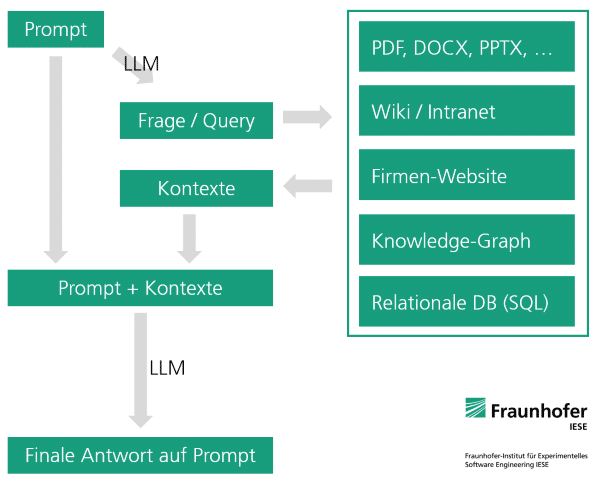
\includegraphics[width=0.5\textwidth]{retrieval_augmented_generation_RAG_600px.png}
    \caption{Struktur eines RAGs, Quelle: \cite{honroth2024retrieval}}
    \label{fig:Rag Structure}
\end{figure}


\subsection{Vorteile von RAGs}
Bei der Wissensabfrage durch LLMs zeigen sich unter anderem folgende Schwachstellen:
\begin{enumerate}
    \item Im Trainingsset für die LLMs selten vorkommendes Wissen können selbst LLMs schlecht lernen. \cite{gao2023rtre} \cite{press2022measuring}
    \item LLMs kennen nur die verwendeten Trainingsdaten und müssen weiter trainiert werden, um neue Informationen zu erlernen.
    \item Firmeninterne Dokumente sind nicht im Trainingsset, und daher können LLMs keine Fragen zu firmeninternen Daten beantworten.
\end{enumerate}

Die Nutzung eines RAGs ist eine der drei Möglichkeiten, um ein LLM zu verbessern. Die anderen beiden Möglichkeiten sind Finetuning und die Verwendung eines LLMs mit einem großen context window.
Die Größe des context windows beschreibt die Menge an Text, gemessen in Tokens, die das LLM gleichzeitig berücksichtigen kann. Ein Token ist ein Teil eines Wortes, ein Wort oder ein Satzzeichen.
RAGs haben neben dem Fine-Tuning und der Nutzung eines LLMs mit großem context window entscheidende Vorteile.

Es gibt einige Faktoren, welche die Entscheidung beeinflussen können, ob ein RAG besser für den betrieblichen Ablauf geeignet ist.
Dazu gehören z. B. die Kompetenz der Betreiber des RAGs, die Art der Daten und die finanziellen Möglichkeiten des Unternehmens.


\subsection{Kompetenz des Betreibers}
Für das Finetuning von LLMs ist technisches Wissen notwendig, um die Themen Natural Language Processing (NLP), Deep Learning, Modellkonfiguration, Datenaufbereitung und Evaluierung anzuwenden.
Der gesamte Prozess des Finetunings ist technisch anspruchsvoll, erfordert das Sichten der neuen Trainingsdaten und ist zudem durch die benötigte Hardware teuer.

Das Benutzen eines LLMs benötigt die geringste Kompetenz des Betreibers, da hier das LLM unverändert bleibt. Hier werden einfach die Daten inklusive der Frage an das LLM gesendet.

Während das LLM in einem RAG auch unverändert bleibt, wird es in ein System mit mehreren Komponenten eingebunden.
Hier ist ein allgemeines Verständnis von LLMs und effektiven Methoden für den suchenden (Retrieval) Teil des RAGs notwendig.
Zudem müssen hier manuell für jedes Dateiformat (E-Mail, PDF etc.) Anbindungen erstellt werden. Sollte ein seltener oder proprietärer Datentyp verwendet werden, muss hier eventuell eigens eine Anbindung entwickelt werden.
\subsection{Datenbasis}
Sollten die Daten dynamisch sein, wie E-Mails, ist das RAG die vorzuziehende Lösung. Dies liegt an den Eigenschaften der schnellen und kontinuierlichen Aktualisierung der Daten.
Wie oben erläutert, kann es jedoch sein, dass es schlechte oder keine Unterstützung von selten verwendeten Dateiformaten gibt.

Der Prozess des Finetunings erstellt hingegen eine Momentaufnahme, die ein erneutes Training erfordert.
Beim Finetuning ist es möglich, dass das Modell Muster erkennt und firmeneigene Begriffe verstehen kann. Dies ist ein deutlicher Vorteil gegenüber den anderen Methoden.


\subsection{Budget}
Das Finetuning erfordert über einen langen Zeitraum teure Rechenzeit auf Hochleistungs-GPUs.
Dabei handelt es sich um spezialisierte Grafikprozessoren, deren Architektur auf die massive parallele Verarbeitung von Daten optimiert ist, was sie für die rechenintensiven Operationen des Machine Learnings, insbesondere neuronale Netze, unerlässlich macht.
Zudem ist die Qualität der Daten entscheidend, ohne das vorherige filtern der Daten durch Menschen ist dieser Prozess aktuell nicht möglich. Sollten sich die Daten als unzureichend erweisen ist die gesammte Rechenzeit verschwendet gewesen.

Das RAG verursacht dagegen zusätzliche Kosten durch das Speichern der Daten in einer Vektordatenbank.

Die wohl kostenintensivste Methode ist die Nutzung eines LLMs mit einem großen Kontextfenster.


\section{Objektive Beurteilung von RAGs}
Je mehr Daten einem RAG zur Verfügung stehen, desto aufwendiger ist es, die Qualität des RAGs zu beurteilen.
Eine Beurteilung durch Menschen müsste bei Anpassungen am RAG oder Änderungen an den Daten neu durchgeführt werden.

Tools wie RAGAS, die bereits eine automatisierte Bewertung versuchen, nutzten bei diesem Prozess unter anderem LLMs.
Diese Tools generieren aus den ihnen gegebenen Daten Fragebögen, die zu einer Frage eine beispielhafte Antwort und die genutzten Stellen aus den vorher gegebenen Dokumenten beinhalten.
Sollten nach diesem automatisierten Test die gewünschten Ergebnisse nicht erreicht werden, kann beispielsweise die Veröffentlichung blockiert werden.

Sowohl menschliche Bewertungen als auch die reine subjektive Bewertung durch LLMs sind jedoch nicht objektiv.
Anhand mehrerer Techniken kann versucht werden, die Bewertung mithilfe von LLMs zu objektivieren. Die Metriken welche Ragas nutzt versuchen z.B. die Anzahl der geannten Fakten aus den Antworten zu extrahieren um so mit Zahlen arbeiten zu können.

\section{Darstellung des Themas und der Forschungsfragen}
In dieser Arbeit soll untersucht werden, wie gut mithilfe von aktuellen RAG-Evualations Tools wie RAGAs RAGs bewertet werden können.
Der Fokus liegt dabei darauf, die Qualität der generierten Fragebögen und der Metriken zu bewerten.

\begin{itemize}
    \item Können RAG-Evaluierungstools wie RAGAS aussagekräftige und kontextrelevante Fragebögen zur Bewertung von RAG-Systemen generieren?
    \item Ermöglichen die durch RAGAS bereitgestellten Metriken und Bewertungen eine valide und zuverlässige Einschätzung der Leistungsfähigkeit von RAG-Systemen?
    \item Zeigen die mit RAGAS durchgeführten Bewertungen signifikante Schwankungen, und welche Implikationen ergeben sich daraus für die Verlässlichkeit der Evaluation?
\end{itemize}


\section{Praxistauglichkeit und Herausforderungen}
Vor Beginn dieser Arbeit antizipierte der Autor bereits Schwierigkeiten bei der Bewertung von Retrieval-Augmented Generation (RAG)-Systemen mittels Ragas
\begin{itemize}
    \item Die Kosten, die bei der Bewertung entstehen.
    \item Die Dauer für die Durchführung der Bewertung. Die Bewertung kann schneller durchgeführt werden, wenn mehr Ressourcen zur Verfügung stehen.
    \item Das Aufsetzen des zu testenden Systems. Dies beinhaltet eine eventuelle doppelte Speicherung der Daten und die für das Testen benötigten Aufrufe des LLMs.
    \item Das System muss auf dem neuesten Stand gehalten werden, da sich dieses aktuelle Thema schnell entwickelt.
\end{itemize}

\section{Softwaretechnische Fragestellungen}

In dem Artikel \textit{RAG in der Praxis – Generierung synthetischer Testdatensätze} untersucht Luka Panic~\cite{pixion2024rag} die Testset-Generierung mithilfe von RAGAS. Es treten bei 17 \% der generierten Fragen Fehler beim Generieren der Testfragen auf.
Dies hat vielfältige Gründe, die von nicht verwertbaren Antworten des LLMs bis zu Verbindungsproblemen oder dem Erreichen des Limits der maximalen Anfragen an APIs reichen.

Auch bei der Bewertung von Antworten können sich ungewollte und bisher noch ungeahnte Biases einschleichen. In dem Paper \enquote{Large Language Models are not Fair Evaluators} \cite{yang2023llmfairness} wird gezeigt, dass, wenn ein LLM eine von zwei gegebenen Antworten aussuchen müsste, die erste bevorzugt wurde, selbst wenn die gleiche Frage mit einer anderer Reihenfolge gestellt wurde.
RAGAS vergleicht keine Antworten miteinander, und daher ist dieser Bias kein direktes Problem für die verwendeten Metriken. Was jedoch einen Einfluss auf die Bewertung von Antworten haben kann, ist der Bias zu gewissen Nummern.
Wie in \cite{shaikh2024cbeval} beschrieben, bevorzugen LLMs bei der Bewertung lieber Zahlen, welche Vielfache von 5 und 10 sind.

Auch die allgemeine stochastische Natur von LLMs spielt eine Rolle, da bei der gleichen Anfrage unterschiedliche Antworten und somit auch Bewertungen zurückgegeben werden. Wie groß diese Abweichungen sind, wird in dieser Arbeit kurz untersucht.

Wie in diesem Paper \cite{gemini2024v15} beschrieben, stellt Gemini 1.5 einen bedeutenden Fortschritt in der multimodalen Verarbeitung großer Kontextfenster dar. Das wirft auch die Frage auf, ob RAGs nicht irrelevant sein könnten und durch LLMs mit großen Kontextfenstern abgelöst werden.
Es gibt einige Gründe, die dagegen sprechen: LLMs mit größeren Kontextfenstern werden immer langsamer und teurer; die genauen Kosten sind abzuwarten. Jedes Mal alle Daten in den Kontext zu laden, besonders wenn dies über das Internet geschieht, ist eine weitere Hürde. LLMs fällt es auch schwer, bei zu vielen Informationen noch die relevanten zu finden, was zu schlechteren Antworten führen kann.
Diese Faktoren lassen darauf schließen, dass RAGs, die nicht nur eine einfache Suche nutzen, noch länger relevant bleiben.

Inzwischen werden spezielle LLMs wie Pleias-RAG entwickelt um die Suche mit RAGs zu verbessern. \cite{huggingface_pleias_rag_1b}
% Kann ich hier wirklich Diskussionen von Twitter linken oder mache ich mich dann lächerlich?
% https://x.com/agishaun/status/1758561862764122191
% https://x.com/ptsi/status/1758511315646320920

% https://huggingface.co/PleIAs/Pleias-RAG-1B

% Pitfalls in LLM Assisted Evaluation https://medium.aiplanet.com/evaluate-rag-pipeline-using-ragas-fbdd8dd466c1

\section{Rechtliche Fragestellungen}

Am 01.08.2024 trat die Verordnung über Künstliche Intelligenz der Europäischen Union (KI-VO) in Kraft. Die Verordnung setzt Regelungen und Maßstäbe für die Verwendung von KI.
RAGs sind gemäß Artikel 3 Nr. 1 KI-VO KI-Systeme und fallen damit in den Anwendungsbereich der KI-VO.
Bei der Nutzung oder Bereitstellung von LLMs muss sich an die KI-VO gehalten werden. Die Nutzer*innen der RAGs müssen sich der aus der KI-VO ergebenden Pflichten bewusst sein.
Ebenso gilt es, bei Anbindung firmeninterner Dokumente, die Datenschutzgrundverordnung zu beachten. Die DS-GVO regelt den Umgang mit personenbezogenen Date, die in solchen firmentinternen Dokumenten enthalten sein könnte.